\documentclass[12pt,a4paper]{scrartcl}
\usepackage[utf8]{inputenc}
\usepackage[ngerman]{babel}
\usepackage{amsmath}
\usepackage{amsfonts}
\usepackage{amssymb}
\usepackage{blindtext}
\usepackage{graphicx}
\usepackage{url}
\usepackage[hidelinks]{hyperref}


\usepackage[left=2.5cm,right=1.5cm,top=2cm,bottom=2.8cm]{geometry}


\usepackage{fancyhdr}
\pagestyle{fancy}

\begin{document}
\begin{titlepage}
\begin{center}

\vspace*{3cm}
\textbf{\huge{Projektarbeit}}\\
\vspace*{2cm}
\textbf{\large{Entwicklung eines 2D-Spiels mit SFML}}\\
\vspace*{5cm}
Gabriel Gavrilas, G3C\\
Jan Kunzmann, G3C\\
Patrick Eigensatz, G3C
\end{center}
\end{titlepage}




\newpage

\setcounter{page}{1}
\section*{Vorwort}


\newpage

\tableofcontents

\newpage

\section{Aufgabenstellung} 
Unsere Aufgabe war eine Projektarbeit zu gestalten. Dazue hatten wir ein Semester Zeit. Man solle ein Thema
wählen, dass einem intressiert. Zu dem eigen ausgewählten Thema muss man etwas erarbeiten, dies dann in einem Lernprotokoll festhalten.
Dazu muss man eine Schriftlichearbeit abgeben und eine Präsentation gemacht werden. Diese Arbeit sollte uns auf die Maturarbeit
vorbereiten.

\subsection{Motivation}
In unserer Generation verbringen viele, vor allem männliche Kinder, Jugendliche und Erwachsene,
ihre Zeit mit dem Spielen von Computer- und Konsolenspielen.
Berühmte Vertreter sind Call of Duty, Grand Theft Auto und Minecraft.
Doch die meisten Nutzer dieser Programme haben nie die Prozesse hinter diesen verstanden.
Sei das wegen der bereits weit fortgeschrittenen Komplexität einiger Spiele 
oder bei einfachen Spielen einfach die fehlende Motivation, sich damit zu befassen.
Viele wollen nur wissen wie man ein Spiel spielt und nicht wie man es spielbar macht.
Da wir selber auch zu dieser Generation gehören, 
haben wir alle Erfahrungen mit verschiedensten "Games".
Doch wir wollten nicht blos Spiele spielen, 
sondern wir wollten selber ein Spiel entwickeln.
Dazu kam noch unsere Begeisterung für den Prozess des Programmierens.
Jeder von uns hatte bereits mehr oder weniger Erfahrungen auf diesem Gebiet gesammelt 
und wir waren und sind alle immer noch bereit mehr zu lernen.

\subsection{Vorgaben}

Vor dem eigentlichen Projekt setzten wir einige Vorgaben.
\\
Uns war klar, dass ein Spiel auf dreidimensionaler Basis in der uns zu Verfügung stehenden Zeit nicht realisierbar war.
Dazu brachte die von uns gewählte Programmiersprache einige Hilfen mit sich, die wir bei der Entwicklung eines 2D-Spiels gut gebrauchen konnten.
\\
Um die Sache für uns attraktiv zu machen,
wählten wir bewusst eine Programmiersprache, die noch nicht
alle von uns beherrschten. Natürlich hätten wir genau so gut
SDL oder direkt das darunterliegende OpenGL verwenden können. OpenGL
schied aus, da der Aufwand bereits ein einfaches 2D-Spiel zu realisieren,
schlichtweg nicht möglich gewesen wäre. SDL war unser Favorit, bis wir
SFML entdeckten. Ganz im Gegensatz zu SDL schien SFML für C++ ausgerichtet
zu sein. So wurden Klassen anstatt Strukturen verwendet, was den (für den
Anfang komplizierten) Umgang mit Zeigern reduzierte. Ausserdem besitzen die
Klassen eigene Konstruktoren, bzw. Destruktoren, was das Initialisieren
oder das freigeben von Speicher überflüssig macht. Davon erhofften wir uns
weniger Speicherzugriffsfehler und ein schnelleres programmieren. SFML
überzeugte uns schlussendlich, als wir die in der offiziellen Dokumentation
gezeigten Beispielprogramme angeschaut haben.

\subsection{Ziele}
\begin{itemize}
\item 
Ziel unseres Projektes ist ein 2D-Einbrecherspiel zu entwickeln. Der Spieler soll eine Figur spielen, die in Häuser einbrechen muss und dort unentdeckt Gegenstände entwenden soll.
\item
Unser persönliches Ziel ist es, durch dieses Projekt, die Anwendung der Techniken der
Programmiersprache C++ zu lernen und zu vertiefen. Dies wollen wir durch
das Prinzip Learning-by-Doing erreichen. Jeder in der Gruppe soll am Ende
mittelgrosse C++-Programme selber programmieren können.
\item
Wir setzen uns zum Ziel,
die Konzepte hinter Frameworks (namentlich SFML) zu verstehen und die
programmiertechnischen Abläufe hinter dem Spiel zu definieren und
umzusetzen.
\item
Wir wollen unser Spiel komplett im Team entwickeln und
mit dem Versionskontrollsystem git vertraut werden. Das alles soll uns später
für eigene Projekte und unsere Maturaarbeit helfen.
\item
Das Spiel muss/soll unter eine OpenSource Lizenz gestellt werden.
\end{itemize}

\newpage
\section{Begriffe}
\subparagraph{Multimedia Framework:}
Eine Bibliothek mit Funktionen, die sich in C++-Programme einbinden lassen. Damit kann man verschiedene Aufgaben plattformübergreifend bewältigen und muss nicht alle Details selber programmieren.

\subparagraph{OpenSource Lizenz:}

Eine Lizenz, die das Einsehen, das Verändern und das Weiterverteilen des Quellcodes erlaubt.

\subparagraph{OpenSource-Software (OSS):}
Software, die unter einer OpenSource-Lizenz verfügbar ist.

\subparagraph{Versionskontrollsystem:}
Ein Programm, das Veränderungen an Dateien aufzeichnet und speichert, sodass mehrere Entwickler den Code gleichzeitig ohne Redundanz verändern können.

\subparagraph{GitHub:}
Für OSS-Entwickler von OpenSource kostenlose Plattform, um die über das Versionskontrollsystem git aufgezeichneten Veränderungen übersichtlich zugänglich zu machen.

\subparagraph{Travis CI:}
Für OSS-Entwickler kostenlose Plattform zur Qualitätssicherung: Kompiliert das Projekt automatisch nach jeder Änderungen und führt Tests durch, um zu sicherzustellen, dass das Programm einwandfrei funktioniert.

\subparagraph{Coverity:}
Für OSS-Entwickler kostenlose Plattform: Führt eine tiefgreifende statische Quellcodeanalyse durch, und hilft so Programmierfehler zu vermeiden und zu finden.

\section{Entwicklungswerkzeuge}
\subsection{SFML}

\subsection{Code::Blocks}
Code::Blocks ist eine frei verfügbare Entwicklungsumgebung (IDE\footnote{Integrated Development Environment}) die Programmierung in C/C++ und D.
Neben der Syntaxhervorhebung und der intelligente Autovervollständigung bietet Code::Blocks bequeme Einstellungen um SFML-Projekte auf allen Plattformen
einfach zu kompilieren. Code::Blocks setzt dabei auf eine Art \textbf{make} wie es schon aus Unixzeiten bekannt ist. Kompiliert wird nur das, was sich
seit dem letzten Durchgang geändert hat. Code::Blocks nutzt \textbf{g++}, den GNU C++ Compiler, um die einzelnen Dateien in Objektcode umzuwandeln und diesen
anschliessen in eine ausführbare Datei zu linken.

\subsection{git / GitHub}
\textbf{git} ist eine sogenannte verteilte Versionskontrolle (DVCS\footnote{Distributed Version Control System}). Ein solches Werkzeug übernimmt
den Entwicklern einige Arbeit, wenn es darum geht, parallel an Software zu schreiben. Zudem zeichnet es alle Änderungen am Code auf und man kann diese
einsehen, um zum Beispiel Fehler zu finden, sie erst seit kurzem vorhanden sind, oder gewisse Änderungen rückgängig zu machen, ohne dass man
manuell die Dateien zerpflücken muss. git überzeugte uns durch seine Einfachheit, seine Effizienz und seine Möglichkeiten. \textbf{GitHub} ist ein
Onlineportal, das das Hosting von Projekten, die mit git verwaltet werden, kostenlos übernimmt. Das Projekt erhält eine eigene Übersichtsseite,
die ebenfalls zur Entwicklung genutzt werden kann, und auf der Interessierte den Code und die Änderungen einsehen können. Wir haben GitHub nicht nur
als Hoster genutzt, sondern ebenfalls, um unsere Termine und Fristen mit dem Projektkalender festzulegen.
\begin{figure}
\centering
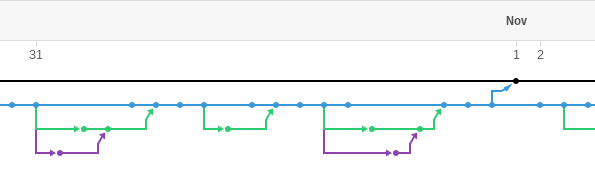
\includegraphics[scale=1]{img/branches.png}
\caption{Verschiedene Entwicklungszweige zur parallelen Entwicklung auf GitHub}
\label{fig:branches}
\end{figure}


\subsection{Coverity Scan}
\textbf{Coverity Scan} ist der Name eines Produktes der gleichnamigen amerikanischen Firma. 2006 erhielt diese Firma vom US-Verteidigungsministerium
einen finanziellen Zuschuss, um es für OpenSource-Projekte kostenlos möglich zu machen, ihren Code auf Sicherheitslücken und Programmierfehler untersuchen
zu lassen. Dabei funktioniert Coverity keines Wegs wie ein normaler Compiler (erkennt also keine syntaktischen Fehler wie das Fehlen eines Semikolons),
sondern es versucht den Code zu verstehen und mögliche semantische Fehler zu finden. So werden Entwickler hingewiesen, dass zum Beispiel eine Funktion
unter gewissen Bedingungen nie terminiert und so das Programm blockiert. Auch findet Coverity schnell Speicherlecks und Speicherzugriffsfehler.
Während der Entwicklung haben wir unser Projekt regelmässig von Coverity überprüfen lassen.
\begin{figure}
\centering
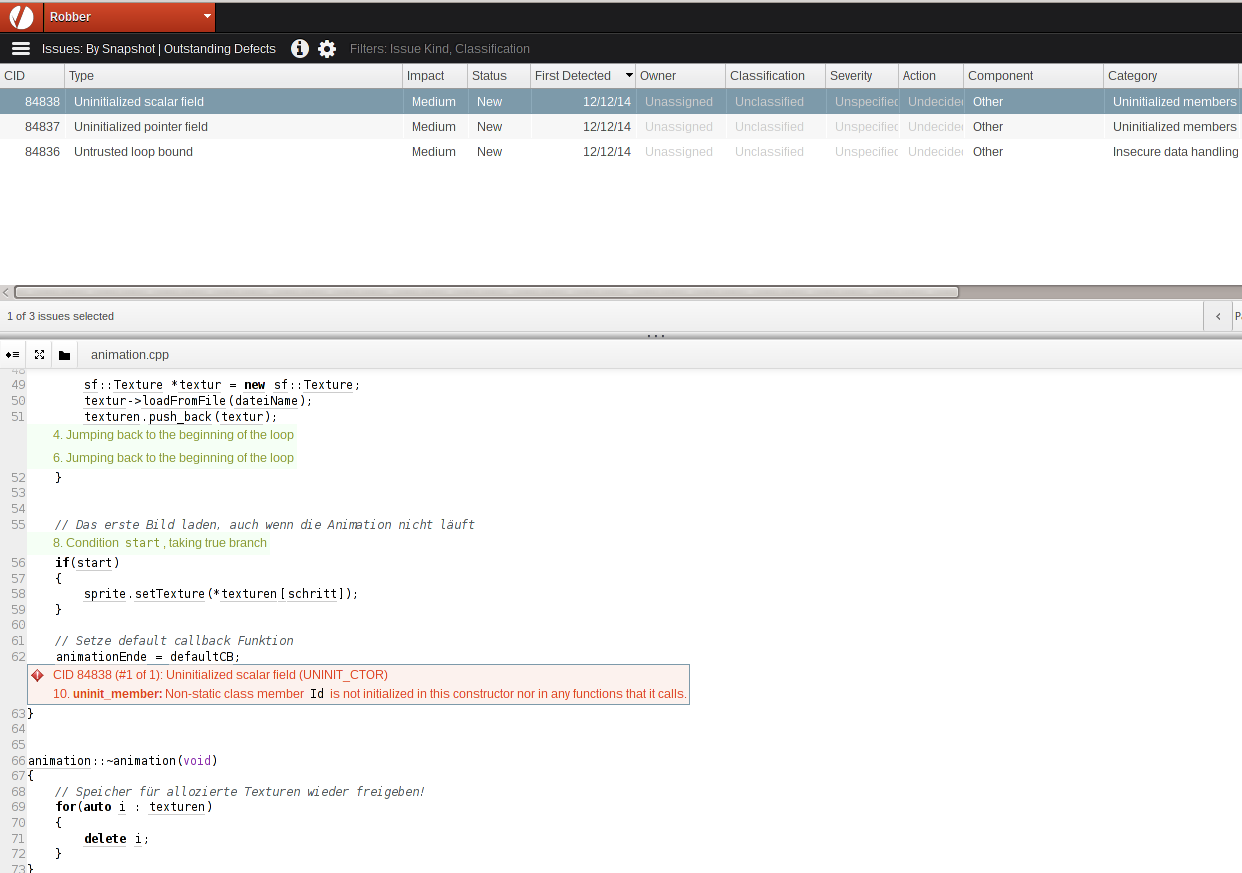
\includegraphics[scale=0.4]{img/coverity.png}
\caption{Coverity hat 3 Fehler gefunden und markiert die fehlerhafte Stelle im Code}
\end{figure}

\subsection{Valgrind}
\textbf{Valgrind} ist ein freies Programm zur dynamischen Fehleranalyse in Programmen. Besonders nutzten wir die Fähigkeit,
unser Spiel innerhalb des Memcheck-Moduls laufen zu lassen, um ein Feedback über den Speicherverbrauch zu erhalten. So entdeckten
wir, dass viele Klassen, die schnell erstellt wurden, zwar Speicher anfordern, diesen aber nie mehr freigeben. Das führte schlussendlich
zu einem Speicherleck von knapp 20MB,
 das schliesslich behoben werden konnte.

\begin{figure}
\centering
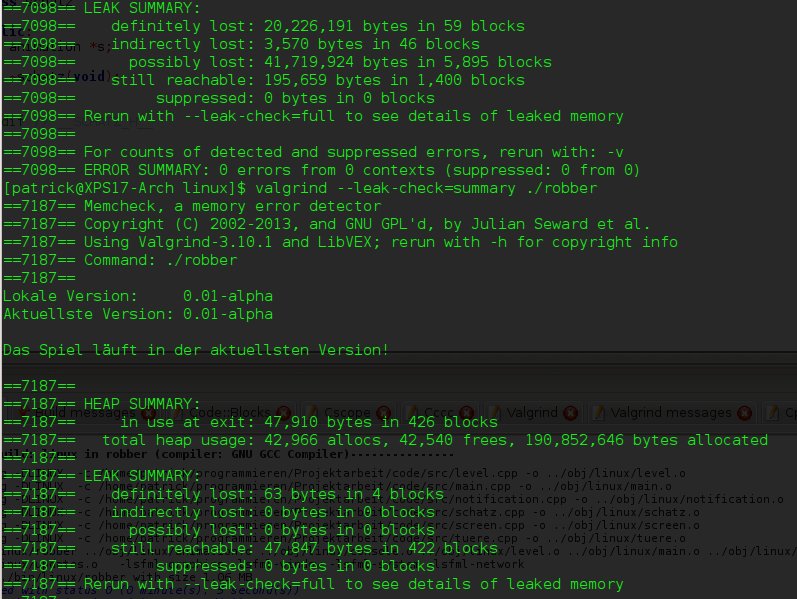
\includegraphics[scale=0.8]{img/valgrind2.png}
\caption{Valgrinds Memcheck}
\end{figure}


\newpage
\section{Vorgehen}
\subsection{Vorbereitung}
\subsubsection{Spielidee}
Am Anfang stand ganz klar die Ideenfindung auf dem Programm. Es war uns wichtig,
eine Spielidee zu finden, an der ein Spieler später auch Spass haben würde,
und wir das Spiel je nach zeitlichen Kapazitäten auch etwas erweitern könnten.
Diese drei Fragen halfen uns:
\begin{enumerate}
\item Würdest du das Spiel spielen?
\item Ist das Spiel technisch überhaupt realisierbar?
\item Ist das Spiel erweiterbar?
\end{enumerate}
Der Ideenfindungsprozess dauerte mehrere Wochen, es war nicht einfach, eine Idee
zu finden, die uns alle begeistern würde. 
Als wir genug Ideen hatten, fertigten wir eine Liste an. 
Wir setzten uns ein Zeitlimit von einer Woche, um zu jeder Idee jeweils einen Umsetzungsvorschlag zu erstellen. 
Dadurch hatten wir zu jeder Idee 3 verschiedene Vorschläge.
Dadurch und durch weitere Diskussion kamen wir auf die Idee eines Eibrecherspiels.
Dieses erfüllte alle Vorgaben:
Die Idee fanden wir alle interessant, es war mit unseren Mitteln und unserem Wissen realisierbar und man kann es gut erweitern.

\subsubsection{Das Planen}
Parallel zur Ideenfindung haben wir uns - wie in der
Disposition vermerkt - intensiv mit der Programmiersprache C++ beschäftigt. Das Einarbeiten
in die Sprache war sehr zentral für das spätere Verständnis der SFML-Bibliothek, die uns
unter Anderem das Anzeigen von Grafiken ermöglichte.
\\
Bevor wir nun jedoch mit dem Programmieren anfangen konnten, mussten wir die Idee ausarbeiten.
Sicher war zuerst nur, dass es ein zweidimensionales Spiel sein wird und das Thema Einbrechen werden soll.
Darum begannen wir das Spiel zu porträtieren. 
Das leeren eines Hauses sollte das Ziel sein, wobei wir damals noch 3 verschiedene Spielmodi geplant hatten:
\begin{enumerate}
\item Einen bestimmten Gegenstand klauen
\item In einer bestimmten Zeit, so viel wie möglich stehlen
\item Einen möglichst hohen Wert der gestohlenen Waren erreichen
\end{enumerate}
Bei den Grafiken einigten wir uns auf Einfachheit, denn es ist kein zentraler Punkt unseres Spieles.
Bereits in diesem Stadium besprachen wir auch mögliche Probleme beim Programmieren und dem Aufbau des Programms.
Dabei wurden die Grundsteine für wichtige Elemente unseres Programms gelegt: Kollisionsdetektion, Teleportieren, Schätze oder auch die Loops, auf denen unser Spiel basiert. 
Durch diese vorhergehende Fehlersuche hatten wir bereits Lösungen zu einigen Problemen, auf die wir treffen würden.
Der nächste Punkt war das Umsetzen unseres gesammelten Wissens und damit das Erstellen des Programms.

\newpage
\subsection{Das Programmieren}
\subsubsection{Das Laden erster Grafiken}
Unsere erste Version des Spieles war bloss ein Fenster mit der Hintergrundgrafik.
Zu allen Dingen haben wir zuerst Demografiken gebraucht.
Obwohl dieser Schritt einfach erscheint kam dabei eines unserer grössten Probleme in der Entwicklung des Spieles zum Vorschein.
Die Schwierigkeit war es, dass diese erste Version bei allen gleich aussieht, unabhängig von Auflösung, Marke oder Betriebssystem.
Weiteres zu diesem Problem gibt es im Kapitel: 5.1 Auflösungsprobleme XY


\begin{figure}[h]
\centering
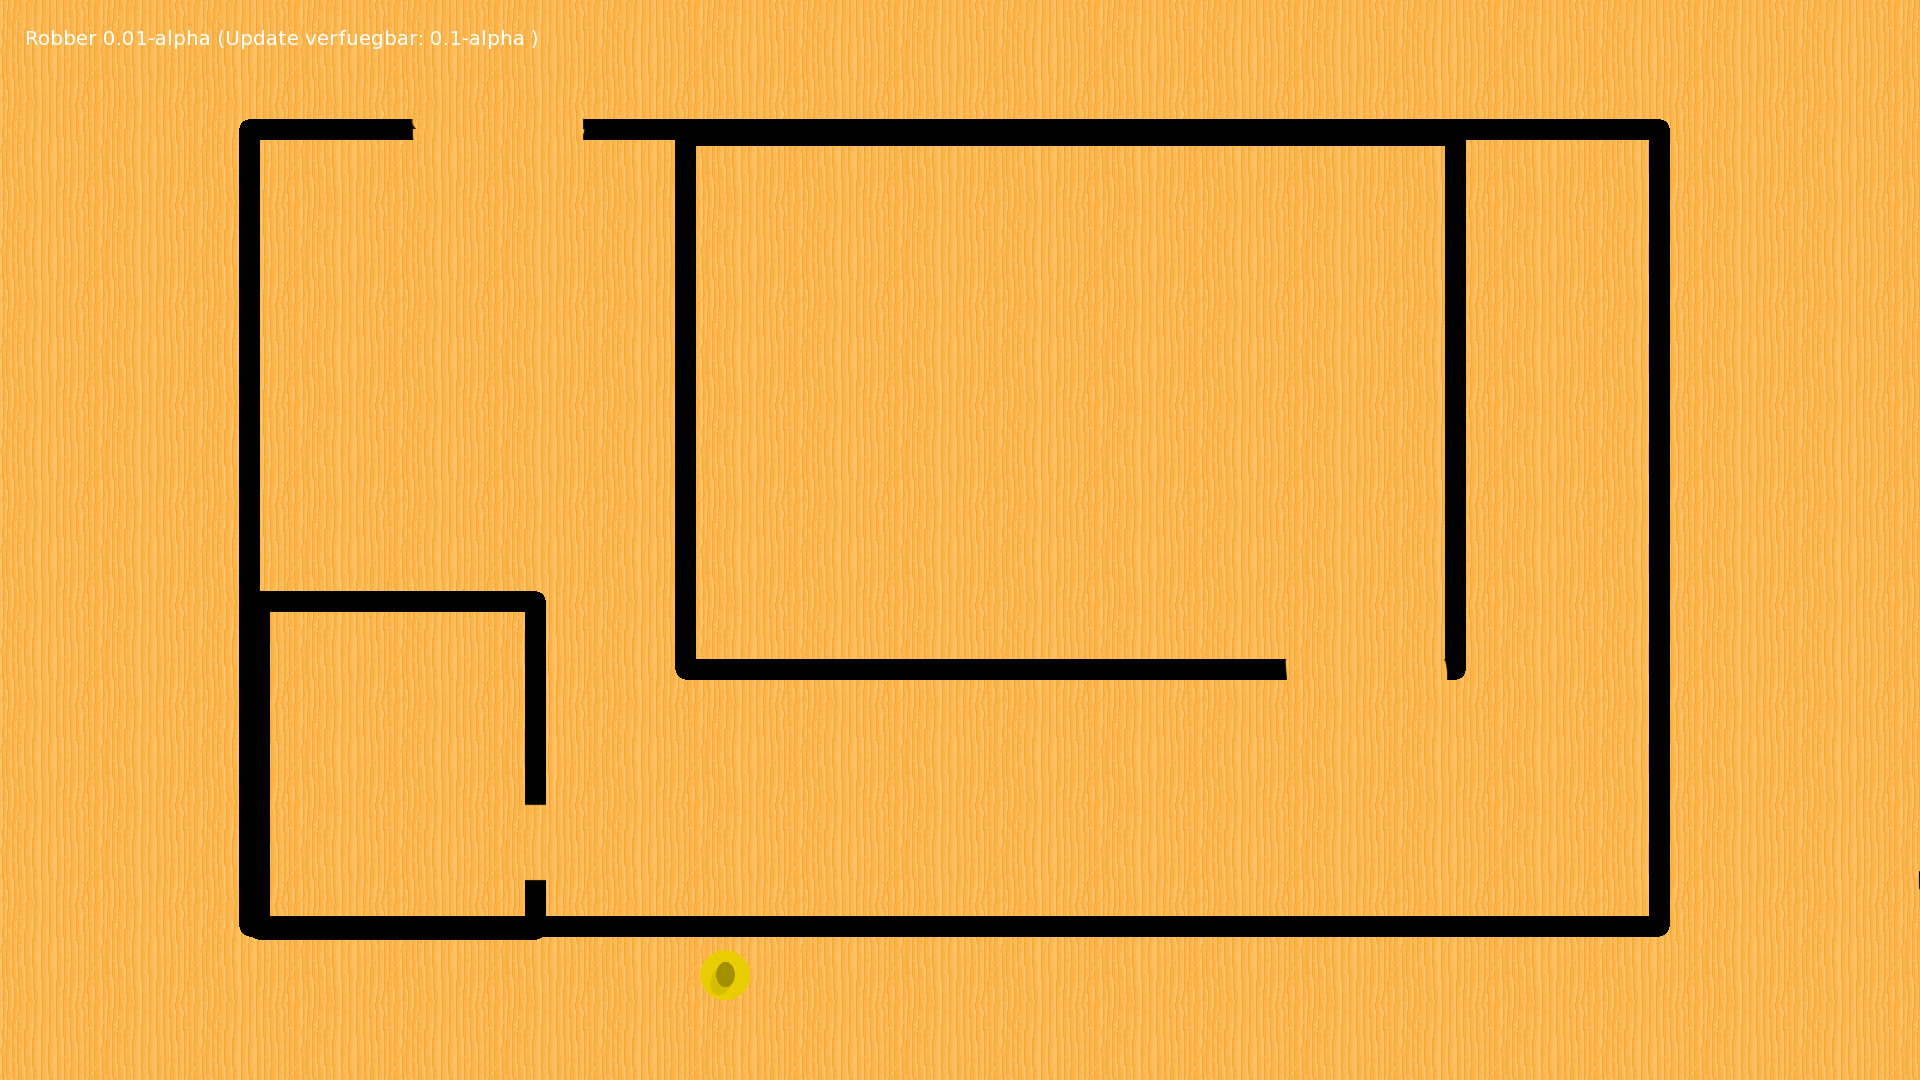
\includegraphics[scale=0.25]{img/grafiken.png}
\caption{Ein Beispiellevel mit der Spielfigur}
\end{figure}
)

\subsubsection{Überprüfung auf Updates}
Versionsdatei von GitHub geladen, wenige Bytes, überprüfen und entsprechende Meldung im Spiel.
Wird noch ausgedeutscht.

\subsubsection{Kollisionsdetektion}
Die Kollisionsdetektion war zu Beginn der Entwicklungen etwas fehleranfällig. So gab es vereinzelt
Schlupflöcher ganz geringer Breite, sodass man durch die Mauer wandern konnte. Neben der Mauer hingegen,
versteckte sich eine unsichtbare Mauer, das heisst, es wurde eine Kollision gemeldet, obwohl an der
Spielerposition gar keine Mauer lag. Um das Problem zu Erforschen und schliesslich zu beheben, haben
wir die Mauerabschnitte einzeln geladen und ein grünes Rechteck darübergezeichnet. So fiel uns auf, dass
die Koordinaten der Mauer zwar richtig gelesen, aber falsch verarbeitet wurden. Die Koordinaten mussten
von absoluten Bildschirmkoordinaten in Fenster/Spielkoordinaten umgerechnet werden. Das konnte wir nach einigem ausprobieren beheben.

\begin{figure}[h]
\centering
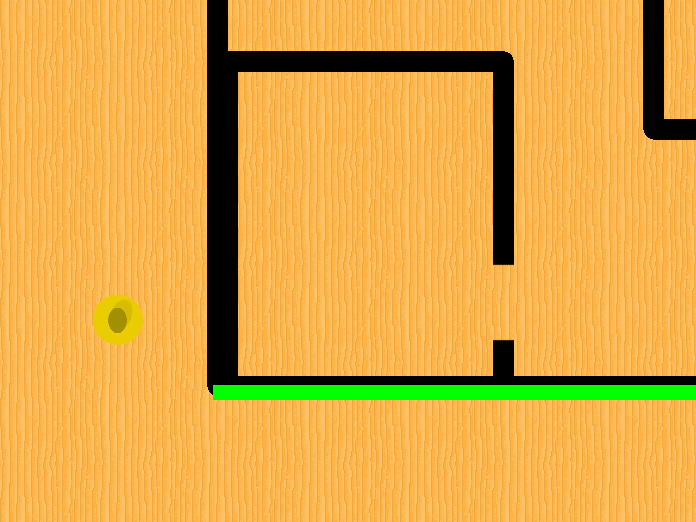
\includegraphics[scale=0.3]{img/kollisionsdetektion.png}
\caption{Debugging der Kollisionsdetektion}
\end{figure}

\subsubsection{Levelclass und Leveldatei}
Unser Ziel war zuerst ein Probe Level zu haben, es dann aber einfach zu haben ein richtiges Level zu erstellen. Deshalb haben wir uns entschieden, dass wir zu jedem Level eine Leveldatei machen, in der alle variablen informationen enthalten sein müssen. So steht dort immer zuerst wie viele, dass es von diesem Obejekt hat und dann oft noch die genaue Position. SO stehen die Mauer oder auch die Pfeile dort vermerkt. Es steht auch zu welchem Level gejumpt werden soll wenn man auf einen Pfeil kommt.
Dies wird in der Leveclass alles genau heraus gelesen. Das wichtige dabei ist, dass die Reihenfolge genau stimmt sonst gerät das ganze in ein irres Durcheinenader. Wir brauchen die Anzahl Elemente die es hat zuerst, um zu erkennen welche Information zu welchem Objekt gehört. Denn das Programm liesst dort nur Zahlen heraus. Und mit Wörtern können wir ihm das nicht erklären, da er diese ja nicht verstehen kann. 

\subsubsection{Animationen}
Von Anfang an waren auch Animationen in unserem Spiel eingeplant. So sollen zum Beispiel ausserhalb eines Hauses
Türen durch grün blinkende/aufleuchtende Pfeile markiert werden. Für solche Animationen wurde eigens eine Klasse
implementiert.
\begin{figure}[h]
	\centering
	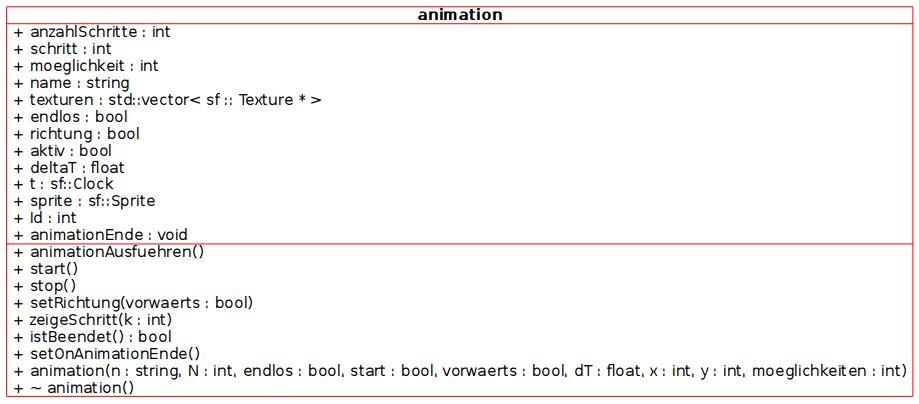
\includegraphics[scale=0.3]{img/animation_uml.png}
	\caption{UML: Animationsklasse}
\end{figure}
Um Animationen später oft und möglichst einfach verwenden zu können, besitzt die Klasse einen einfachen Konstruktor,
der die Bilder bereits lädt, die Position und die Zeitspanne $\Delta t$ zwischen den einzelnen Bildern festlegt.
\begin{figure}[h]
	\centering
	
\includegraphics[scale=0.3]{img/animation_pfeil.png}
	\caption{Die erste Animation im Spiel: Ein blinkender Einstiegspfeil}
\end{figure}
Innerhalb unserer $main()$-Funktion nützten wir eine $std::list<animation *>$ Liste aus der STL\footnote{Standard Template Library}.
Bevor die Sprites in das Fenster gezeichnet werden, werden die Texturen der Sprites dem Animationszeitpunkt entsprechend
neu geladen. So entsteht das Gefühl einer Bewegung, bzw. hier Anpassung der Farbe. Entscheidend ist dabei die Methode
$animationAusfuehren()$, die überprüft, ob bereits genug Zeit vergangen ist, das neue Bild anzuzeigen und dies gegebenenfalls
übernimmt.


\subsubsection{Türen}
Das mühsamste beim Implementieren der Türen waren die dynamischen Mauern. Zwar kann die Mauer Liste mit den
STL-Funktionen $push\_back()$ und $remove()$ einfach hinzugefügt, bzw. entfernt werden, jedoch muss die Mauer
immer entsprechend umgerechnet werden. Dies ist besonders bei den 4 verschiedenen möglichen Rotationen etwas mühsam.
Auch hier haben wir eine checkCollision überprüfung gemacht. So wird überprüft, o der Spieler in der Nähe der Türe ist. Wenn dies der Fall ist wird die Animation gestartet und im Spiel sieht man wie sich die Tür öffnet. Dann wird hier wieder mit den neuen Koordinaten eine „Mauer“ erstellt, die nicht passiert werden kann. Wir haben einen mindest Zeitabstand eingebaut, so dass sich die Tür erst wieder nach einer gewissen Zeit schliessen lässt. Sonst hätte man die Türe schneller öffnen  und schliessen können als das Spiel mithalten könnte und würde die Tür noch oft öffnen und schliessen.Wir haben die Türen noch etwas grösser gemacht bei der Collisions-Abfrage, so dass man die Türen schlussendlich immer von beiden Seiten öffnen und schliessen kann.

\subsubsection{Das Hauptmenü}
Das Hauptmenü wurde bewusst relativ simpel gehalten und konnte dadurch sehr schnell erstellt werden. Mit GIMP wurden
einige mehr oder weniger gut aussehende Grafiken erzeugt, die als Buttons verwendet werden konnten. Doch da wir hier wieder auf ein Problem mit den Koordinaten stiessen entschieden wir uns unser Game nicht, wie viele andere aufzubauen. Nun ist man bereits im Hauptmenu die Spielfigur  und da hatten wir es leicht. Wir haben einfach das Spielstarten Bild als neuen Pfeil definiert falls eine 2 in der Leveldatei steht. So ist es, sobald man auf das Spielstarten fährt einn Teleporter zum ersten Level. Bei der Spielbeenden haben wir ein FloatRect erstellt und eine checkCollison gemacht und falls der Spieler nun auf Spielbeenden fährt beendet das Spiel. 
\begin{figure}
\centering

\includegraphics[scale=0.3]{img/hauptmenu.png}
\caption{Das Hauptmenü}
\end{figure}

\subsubsection{Dunkle Level}
Mit einem halbtransparenten Overlay können wir das Level, bzw. das Haus abdunkeln, und nur in einem Bereich um uns
sichtbar machen. In der Leveldatei wird eingetragen, ob ein Level dunkel, oder hell ist. Dementsprechend wird dann das
Overlay geladen oder nicht. Das führt zu spannenderen Spielen, weil man Gefahren und die Schätze relativ spät sehen kann.
Besonders beim Spiel auf Zeit entsteht so quasi ein zusätzlicher Druck.

\begin{figure}[h]
\centering
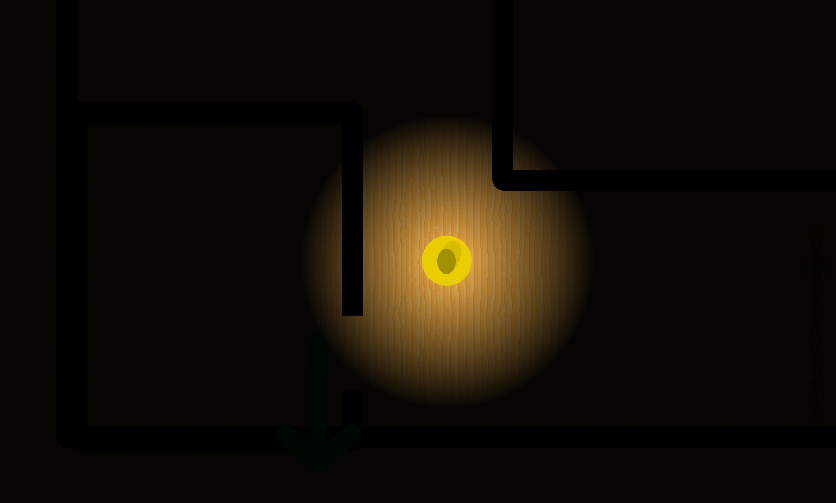
\includegraphics[scale=0.5]{img/dunkel.png}
\caption{Ein dunkles Level}
\end{figure}
\newpage


\section{Probleme und Lösungen}
\subsection{Auflösungsproblem XY}
Beim Auflösungsproblem handelt es sich um ein Problem mit dem Umgang mit SFML.
Das Problem besteht darin, dass jede Ansicht bei jeder Auflösung, jeder Gerätemarke und bei beiden Betriebssystemen gleich aussehen soll.
Wir hofften, dass SFML diese Arbeit übernehmen würde, doch bereits bei den ersten Grafiken mussten wir einsehen, dass wir alles selber regeln müssten.
Um das Problem zu lokalisieren benutzten wir die $zoom()$ funktion, mit der man die ganze Ansicht über einen Wert anpassen kann.
Diesen Wert nannten wir $factor$.
\subsection{Compilerprobleme}
Nicht nur wir machten Fehler bei der Entwicklung, und die Fehler von anderen sind erfahrungsgemäss schwerer aufzuspüren.
Einem eher speziellen Problem begegneten wir, als wir den Pfad für ein Animationsbild erstellen wollten.
Die Zahl $i$, die bei zu zählen anfängt, zeigt, den wievielten Schritt der Animation gerade geladen werden soll, und $n$ steht für den Namen der Animation.
Ein solcher Pfad lautet zum Beispiel für einen\\Pfeil im 4. Animationsschritt: \textit{resources/pfeil\_3.png}\\
\\
In C++11 sind die + Operatoren zum Verketten (Engl. concatenate) von Strings überladen. Damit man auch Zahlen so in Strings einsetzen
kann gibt es seit C++11 die Funktion $to\_string()$, die überladen für sämtliche Zahldatentypen existiert und das Argument in einen String
umwandelt. Der Code kompilierte auf Linux mit dem GNU C++ Compiler (G++) v4.9 ohne Probleme. Als Gabriel und Jan versuchten den Code auf ihrem Windowssystemen
mit dem für Windows aktuellen MinGW G++ v4.7.1 zu kompilieren scheiterte dies. Spannende Recherchen ergaben, dass es sich um einen bei MinGW
gemeldeten Bug\footnote{\url{https://gcc.gnu.org/bugzilla/show_bug.cgi?id=52015}} handelt, der ein Auffinden der Funktion in der unter Windows verwendeten
Version unmöglich macht. Glaubt man den Kommentaren zum Bug, so findet der Präprozessor den Header zwar, liest ihn aber auf Grund eines Guardtokens nicht ein.
Die Funktion ist folglich in der libstdc++ implementiert, wird aber in keinem Header deklariert.\\ %nur leicht unklar für unwissende...
\\
Ein Lösungsansatz wäre gewesen, die in C für diesen Zweck bestimmte Funktion \textit{sprintf()} zu nutzen, dies hätte jedoch einen C-String zur Folge gehabt.
Da wir am Anfang C++ als Programmiersprache wählten, um den C-Problemen wie Speicherverwaltung, C-Strings, etc. aus dem Weg zu gehen, entschieden wir uns, über
Präprozessorflag (\textit{\#ifndef}) das \textit{LINUX}-Makro zu prüfen. Existiert dieses, so wird die to\_string()-Funktion, ansonsten ein stringstream, verwendet.
Der Commit \textit{e419eef} behebt und dokumentiert genau dieses Problem. Um uns auch später, also während der Erstellung der Dokumentation, einen Überblick
über die behandelten Probleme verschaffen zu können, haben wir diese in den Commits jeweils kurz erläutert. Das genannte Problem findet sich im
Konstruktor der Animationsklasse, in der Datei \textit{code/src/animation.cpp}.


\begin{figure}[h]
\centering
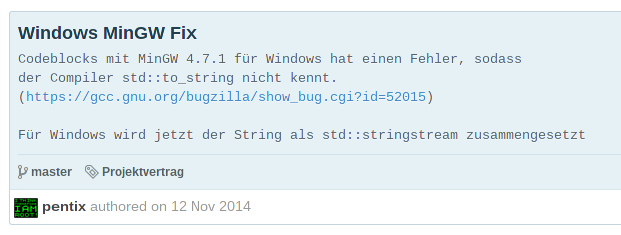
\includegraphics[scale=0.8]{img/e419eef.png}
\caption{Erläuterung in einem Commit}
\end{figure}

\subsection{Merge Conflicts}
git, unsere Versionskontrolle, ermöglichte es uns, parallel, in sogenannten Branches zu entwickeln. (Siehe Abbildung \ref{fig:branches} auf Seite \pageref{fig:branches}). Wir entwickelten neue Funktionen oft parallel und "mergten" (engl. to merge = zusammenführen) sie in unseren master-Zweig.
git nimmt alle Änderungen, die in beiden Zweigen seit dem letzten gemeinsamen Commit erstellt wurden, und erstellt daraus neue Dateien, die alle Änderungen,
also die Änderungen von beiden Zweigen beeinhalten. Es kann sein, dass nun 2 Personen gleichzeitig an derselben Stelle im Code etwas geändert haben. Zum Beispiel
hat der eine Entwickler eine Abfrage gelöscht, weil er sie nicht mehr brauchte, ein anderer Entwickler hat jedoch dieselbe Abfrage erweitert, da er sie benötigt.
git kann nun nicht mehr automatisch entscheiden wie der Code zusammenzuführen ist, bzw. wie die Versionen kombiniert sein sollen. Daraus resultiert ein Merge
Conflict. Git erstellt eine Datei, in der beide Versionen der Entwickler vorhanden sind und bittet den Entwickler, der den Code des anderen in seinen führen
will, um Hilfe. Unsere Konflikte waren meistens schnell gelöst, da sie nur zwei bis drei Zeilen betrafen, zum Beispiel wurde bei beiden Entwicklern
eine Variable unbenannt und man musste entscheiden, welche Version man wählt.\\
\\
Mühsam hingegen waren Konflikte, die mehrere Dateien betrafen, und in der 20 bis 30 Zeilen in einem Klammerwirrwar in Konflikt stehen. Da die Dateien und die Zeilen
logisch voneinander abhängen, musste man sehr umsichtig sein, und brauchte entsprechend viel Zeit und Geduld einen solchen Konflikt zu lösen. Es gab zum Glück kein
grosser Konflikt, der uns Probleme bereitete.
\newpage

\subsection{Paralleles Entwickeln des Kerns}
Obwohl wir bereits am Anfang parallel mit git entwickeln konnten, war es sehr schwierig, da noch gar kein Code vorhanden war,
und es zuerst galt, eine Basis zu entwickeln, auf der dann alle Programmieren konnten. Wir versuchten von Anfang an so zu programmieren,
dass wir später keine grossen Änderungen vornehmen mussten, um das Spiel um Laserschranken oder auch Musik zu erweitern.
\\
\\
Das gelang uns sehr gut, einzig die Levelklasse brauchte eine Restrukturierung, da die \textit{loadFromFile()}-Methode eine Leveldatei nicht nur mehr auslas,
sondern die Objekte auch gleich zeichnete. Da wir die Level aber speichern und nicht immer mehr komplett neu laden wollten, brauchten wir eine
Funktion, die es uns ermöglichte nur die Objekte in die Levelklasse zu laden und eine Funktion, die nur dazu da war, die gespeicherten Objekte zu zeichnen. So konnten wir Veränderungen an den Objekten in der Levelklasse abspeichern.
\\
\\
Ansonsten mussten wir am ganzen Kern nichts mehr ändern. Der grosse Vorteil, der sich dadurch ergab, war, dass jeder seine 
Funktionen kannte, und zum Beispiel problemlos Objekte erstellen konnte und diese auch auf Kollisionen mit dem Spieler überprüfen konnte.

\subsection{Mathematik}
Aufwand zum berechnen/ Logik

\subsection{Verfügbare Zeit}
Am Anfang des Projektunterrichts dachten wir, wir hätten mehr Zeit für die eigentliche Entwicklung. Wir mussten schlussendlich aber auch
sehr viel Zeit in die Disposition, den Projektvertrag und das Lernprotokoll stecken. Die Zeit, die uns für die Dokumentation und das Spiel
blieb, haben wir aber sehr intensiv genutzt. Die Kreise in Abbildung \ref{fig:punchcard} zeigen additiv, wie viel und wann seit Projektbeginn programmiert wurde.

\begin{figure}[h]
\centering
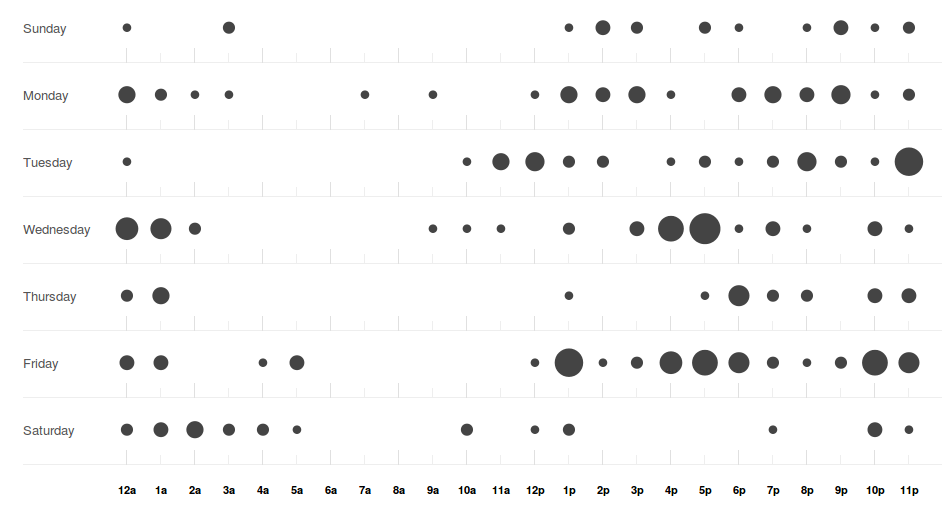
\includegraphics[scale=0.4]{img/punchcard.png}
\caption{Punchcard - Darstellung der Entwicklungszeiten}
\label{fig:punchcard}
\end{figure}

\section{Das Spiel}
\newpage
\section{Diskussion / Reflexion}

\newpage
\section{mögliche Erweiterungen / Ausblick}

\clearpage
\listoffigures
\end{document}
